\documentclass{article}

\usepackage{amsmath}

\usepackage{pgfplots}
\usetikzlibrary{calc}

\pagestyle{empty}

\begin{document}

Your function can be plotted symmetrically in the coordinate system defined by
the principal axes of the ellipse. Your function is minimized at $x=x_0=19/10$ and 
$y=y_0=9/5$ with $f(x_0,y_0)=-10.1=:z_0$. So the first step is a translation
\[ x'~=~x-x_0\;,\quad y'~=~y-y_0\quad\text{and}\quad
z'~=~z-z_0\;.\]
The second step is to rotate to the principal axes, which can be achieved by
diagronalizing the Hesse matrix of $f$,
\[
 H~=~\begin{pmatrix} 4 &  -2\\ -2 &  6\end{pmatrix}\;.
\]
This yields a rotation angle of $31.8^\circ$. The perhaps simplest way to
produce the figure is thus to plot the function in the principal axes system and
draw the unrotated axes by hand.

\begin{center}
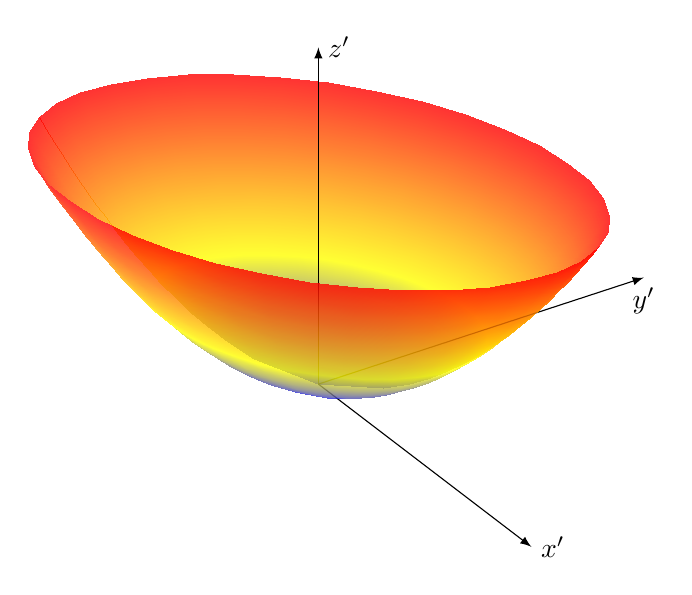
\begin{tikzpicture}
\begin{axis}
[
%view={135}{45},
%colormap/blackwhite, 
axis equal,
width=12cm,
axis lines=center, axis on top,
axis line style={draw=none},
ticks=none,
set layers=default,
domain=0:1.50,
samples=20, % this was 200, but I changed it to 20 because of my slow PC
z buffer=sort,
]
\addplot3 [surf,shader=interp,opacity=0.8,
domain y=0:180] ({1.62*cos(y)*sqrt(x)},{sin(y)*sqrt(x)},{x});
\addplot3 [surf,shader=interp,opacity=0.8,
domain y=-180:0,on layer=axis foreground] ({1.62*cos(y)*sqrt(x)},{sin(y)*sqrt(x)},{x});
\coordinate (O) at (axis cs: 0,0); 
\def\AxLen{2.5}
\coordinate (oriX) at (axis cs: {\AxLen*cos(-31.8)},{\AxLen*sin(-31.8)});
\coordinate (oriY) at (axis cs: {-\AxLen*sin(-31.8)},{\AxLen*cos(-31.8)});
\coordinate (oriZ) at (axis cs: 0,0,\AxLen*1);
\coordinate (realO) at ($-{19/10}*(oriX)-{9/5}*(oriY)$);
\end{axis}
\draw[-latex] (O) -- (oriX) node[right]{$x'$};
\draw[-latex] (O) -- (oriY) node[below]{$y'$};
\draw[-latex] (O) -- (oriZ) node[right]{$z'$};
\end{tikzpicture}
\end{center}

\end{document}
